%! TEX root = main.tex

For the steady cases, the PINN solver took about 25 hours to finish for $N_{bs}=\num{25600}$ and 13.5 hours for $N_{bs}=\num{6400}$.
The unsteady PINN solver, on the other hand, took about 26 hours and 14.5 hours for $N_{bs}=\num{25600}$ and $\num{6400}$, respectively.
The baseline PetIBM simulation was finished within 2 minutes.

Figure \ref{fig:cylinder-2d-re40-loss-hist-steady} shows the convergence history of the aggregated losses for the steady cases, and figure \ref{fig:cylinder-2d-re40-loss-hist-unsteady} shows those for the unsteady cases.
Each figure includes sub-figures for losses against iterations and run times.
\begin{figure}[hbt!]
    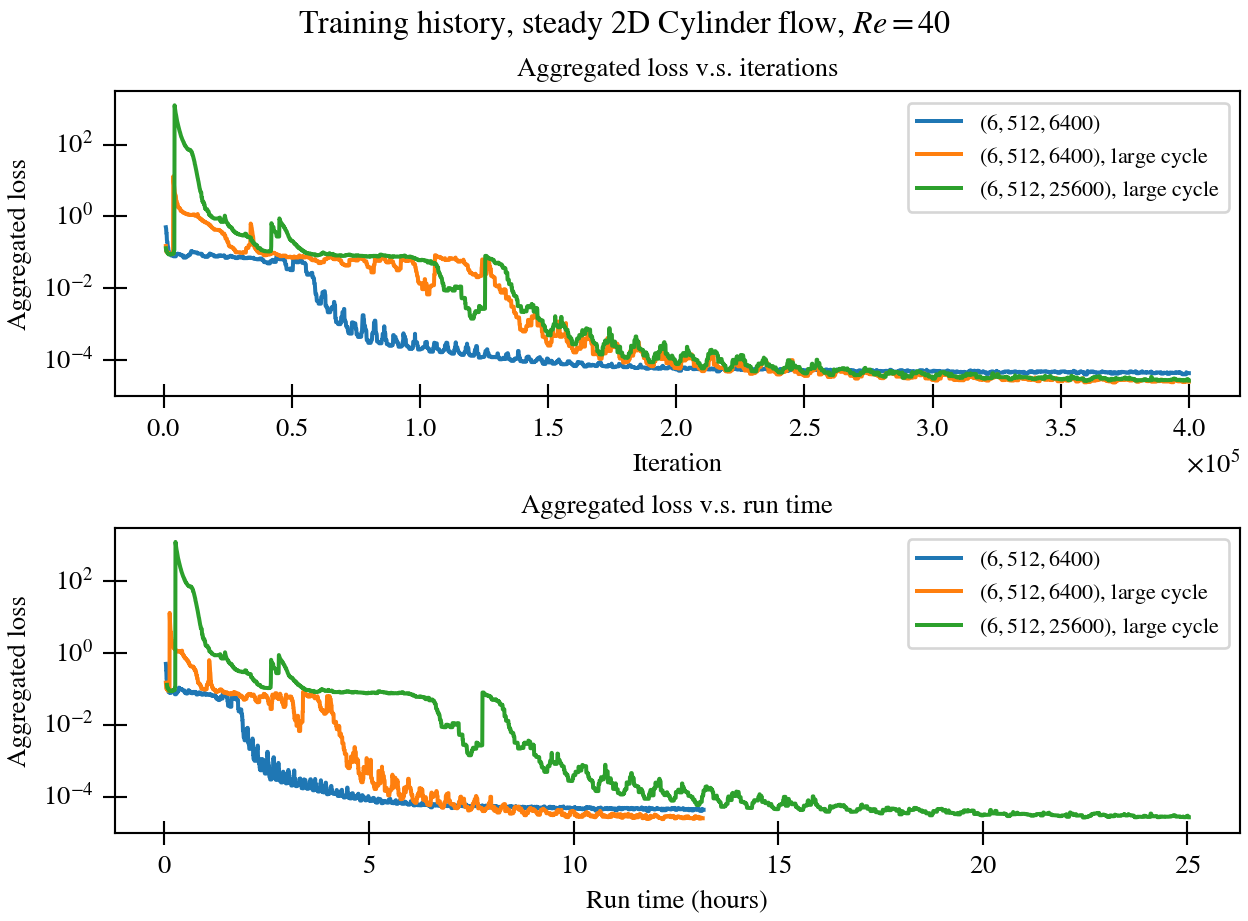
\includegraphics[width=0.9\linewidth]{cylinder-2d-re40/loss-hist-steady}
    \caption[%
        PINNs, 2D Cylinder, $Re=40$: training history of steady solvers%
    ]{%
        PINNs, 2D Cylinder, $Re=40$: training history of steady solvers%
    }%
    \label{fig:cylinder-2d-re40-loss-hist-steady}
\end{figure}
\begin{figure}[hbt!]
    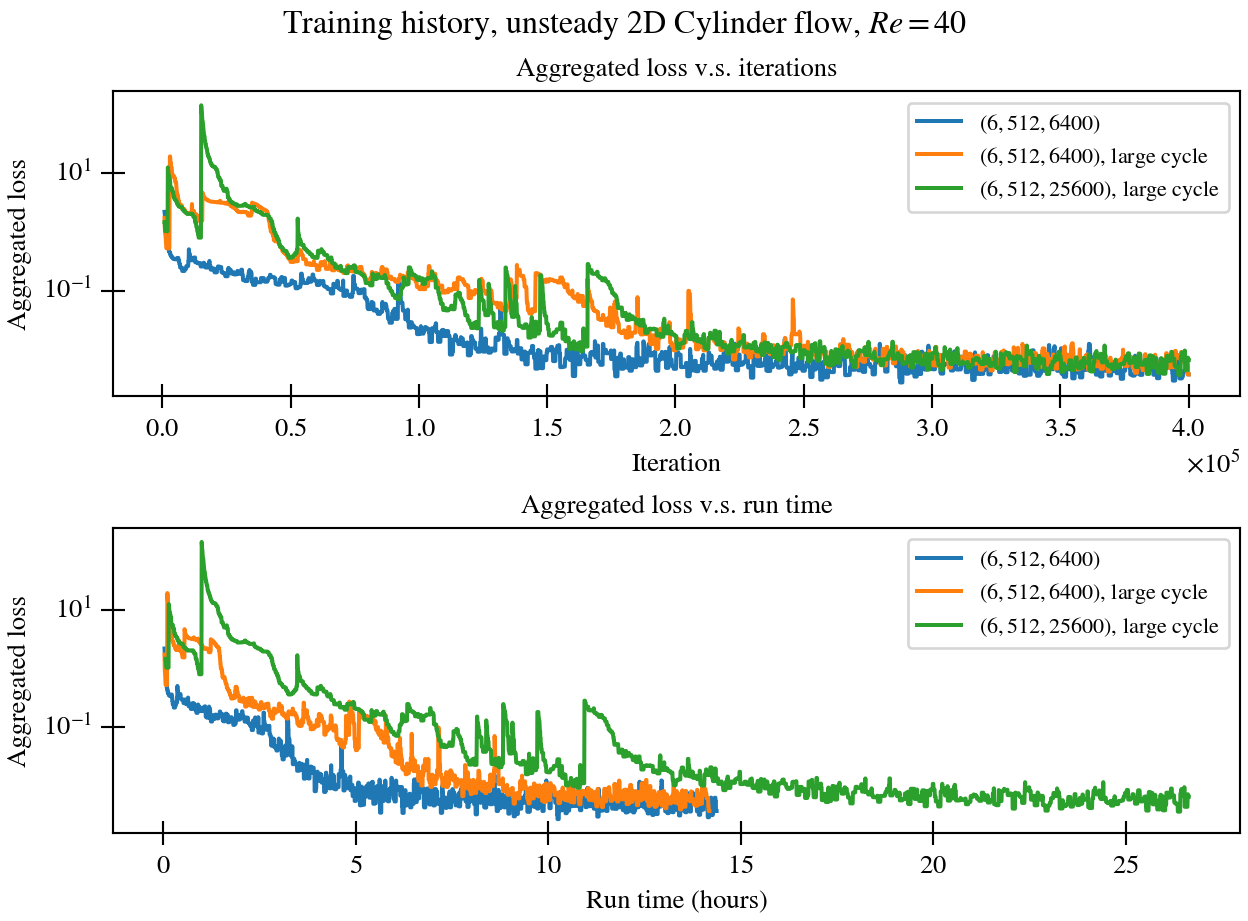
\includegraphics[width=0.9\linewidth]{cylinder-2d-re40/loss-hist-unsteady}
    \caption[%
        PINNs, 2D Cylinder, $Re=40$: training history of unsteady solvers%
    ]{%
        PINNs, 2D Cylinder, $Re=40$: training history of unsteady solvers%
    }%
    \label{fig:cylinder-2d-re40-loss-hist-unsteady}
\end{figure}
An interesting observation from figure \ref{fig:cylinder-2d-re40-loss-hist-steady} is the plateaus at the beginning of the training.
Though without a proof, we suspect this trend reflects the escaping from saddle points.
The large cyclical schedule took more time to escape because it had fewer cycles under given iterations.
Regardless of the difference at the beginning, all cases reached the same level of losses eventually.
And for the large cyclical schedule, both $N_{bs}=\num{6400}$ and $N_{bs}=\num{25600}$ show similar convergence history in terms of iterations.
This observation again substantiates our suspicion in the previous section that $N_{bs}$ does not have significant influence on the losses and errors.

Figure \ref{fig:cylinder-2d-re40-loss-hist-unsteady} also shows plateaus at the beginning, though not as obvious as those for the steady cases.
The convergence histories for the unsteady cases are also bumpier.
We also suspect that it is caused by escaping from saddle points and poor local minimums.
The hypersurface of the unsteady solver might be more complicated than the steady one, hence causing more oscillating convergence.
Nevertheless, all unsteady cases converged to a similar loss level.

Figure \ref{fig:cylinder-2d-re40-contours} shows visual comparisons of the steady-state flow fields.
\begin{figure}[hbt!]
    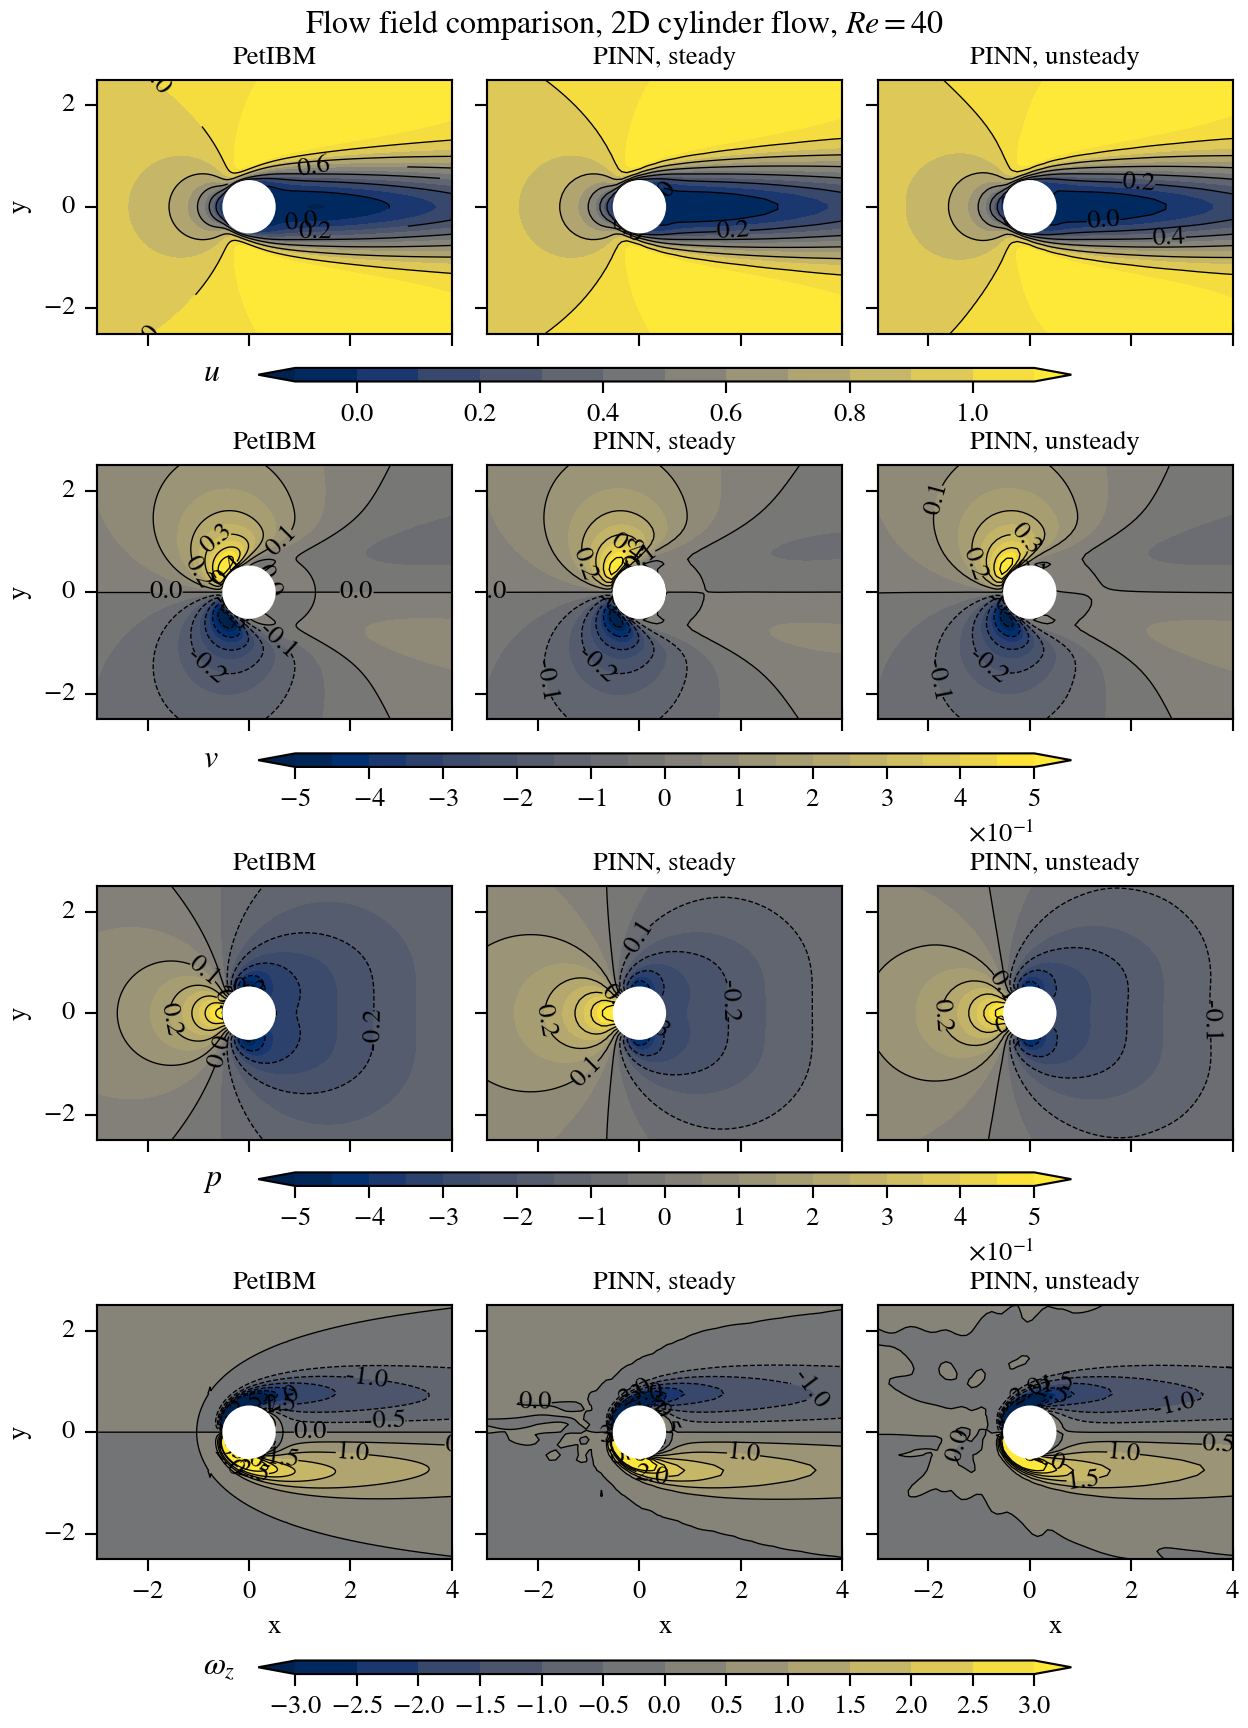
\includegraphics[width=\linewidth]{cylinder-2d-re40/contour-comparison}
    \caption[%
        PINNs, 2D Cylinder, $Re=40$: flow fields at steady state%
    ]{%
        PINNs, 2D Cylinder, $Re=40$: flow fields at steady state. %
        For the unsteady PINN case, the solution was extracted from $t=20$. %
        The fields shown, from the top to bottom, are $u$, $v$, $p$, and vorticity $\omega_z$.%
    }%
    \label{fig:cylinder-2d-re40-contours}
\end{figure}
The results of steady PINN solver were obtained from the case of $N_{bs}=\num{25600}$ with the large cyclical schedule, and that of the unsteady solver was also obtained from the same $N_{bs}$ and schedule.
All three cases visually agree with each other, except for the vorticity.
Note that vorticity is obtained by post-processing for all three solvers.
PetIBM relies on central difference to calculate the vorticity, while PINNs use automatic differentiation to obtain it.

Figure \ref{fig:cylinder-2d-re40-drag-lift-time} gives the drag and lift coefficients ($C_D$ and $C_L$).
We only plotted the results from the unsteady solver because the steady solvers do not have the time variable. 
\begin{figure}[hbt!]
    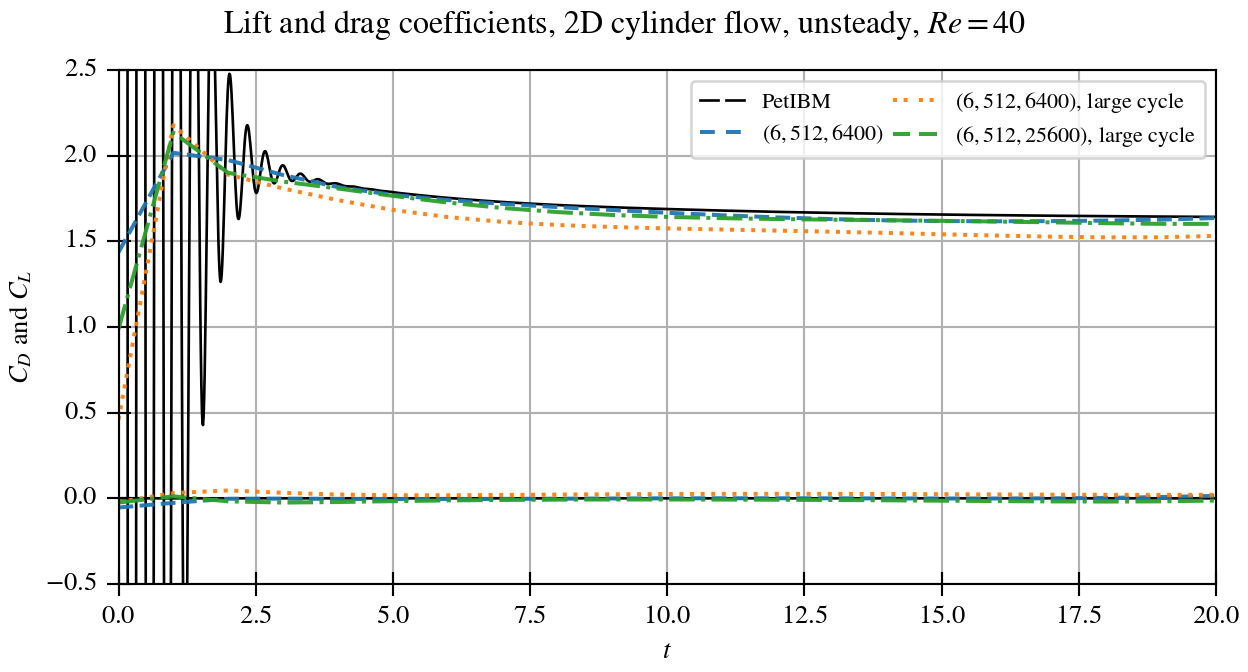
\includegraphics[width=\linewidth]{cylinder-2d-re40/drag-lift-coeffs.png}
    \caption[%
        PINNs, 2D Cylinder, $Re=40$: drag and lift coefficients%
    ]{%
        PINNs, 2D Cylinder, $Re=40$: drag and lift coefficients%
    }%
    \label{fig:cylinder-2d-re40-drag-lift-time}
\end{figure}
Table \ref{table:cylinder-2d-re40-comparison-cd} compares the values of $C_D$ against the experimental data and simulation data from other groups.
\begin{table}[hbt!]
    \singlespacing
    \begin{threeparttable}[b]
        \begin{tabular}{lccc}
            \toprule
            & $C_D$ & $C_{D_p}$ & $C_{D_f}$ \\
            \midrule
            $(6, 512, 6400)$, steady & 1.62 & 1.07 & 0.55 \\
            $(6, 512, 6400)$, unsteady & 1.63 & 1.02 & 0.61 \\
            $(6, 512, 6400)$, large cycle, steady & 1.62 & 1.07 & 0.55 \\
            $(6, 512, 6400)$, large cycle, unsteady & 1.53 & 0.96 & 0.57 \\
            $(6, 512, 25600)$, large cycle, steady & 1.62 & 1.06 & 0.55 \\
            $(6, 512, 25600)$, large cycle, unsteady & 1.60 & 1.06 & 0.55 \\
            PetIBM & 1.63 & 1.02 & 0.61 \\
            Rosetti et al., 2012\cite{rosetti_urans_2012}\tnote{1} & 1.74\pm 0.09 & n/a & n/a \\
            Rosetti et al., 2012\cite{rosetti_urans_2012}\tnote{2} & 1.61 & n/a & n/a \\
            Sen et al., 2009\cite{sen_steady_2009}\tnote{2} & 1.51 & n/a & n/a \\
            Park et al., 1988\cite{park_numerical_1998}\tnote{2} & 1.51 & 0.99 & 0.53 \\
            Tritton, 1959\cite{tritton_experiments_1959}\tnote{1} & 1.48--1.65 & n/a & n/a \\
            Grove et al., 1964\cite{grove_experimental_1964}\tnote{1} & n/a & 0.94 & n/a \\
            \bottomrule
        \end{tabular}%
        \begin{tablenotes}
            \footnotesize
            \item [1] Experimental result
            \item [2] Simulation result
        \end{tablenotes}
        \caption[PINNs, 2D Cylinder, $Re=40$: validation of drag coefficients]{%
            Validation of drag coefficients.%
            $C_D$, $C_{D_p}$, and $C_{D_f}$ denote the coefficients of total drag, pressure drag, %
            and friction drag, respectively.%
        }%
        \label{table:cylinder-2d-re40-comparison-cd}
    \end{threeparttable}
\end{table}%

As seen from the table, values from different previous works in the literature show a variability in $C_D$.
Though there is not a correct answer to compare against, at least the $C_D$ from PINNs and PetIBM all fall into the range of others' works.
And the differences seen in figure \ref{fig:cylinder-2d-re40-drag-lift-time} are acceptable given that the $C_D$ shown in the table are all within the acceptable range.
We consider the results of $C_D$ validated.

Lastly, we compared the pressure coefficient ($C_p$) on the cylinder surface.
Figure \ref{fig:cylinder-2d-re40-surface-cp-steady} shows the surface $C_p$ of the steady cases, and figure \ref{fig:cylinder-2d-re40-surface-cp-unsteady} shows that of the unsteady cases.
\begin{figure}[hbt!]
    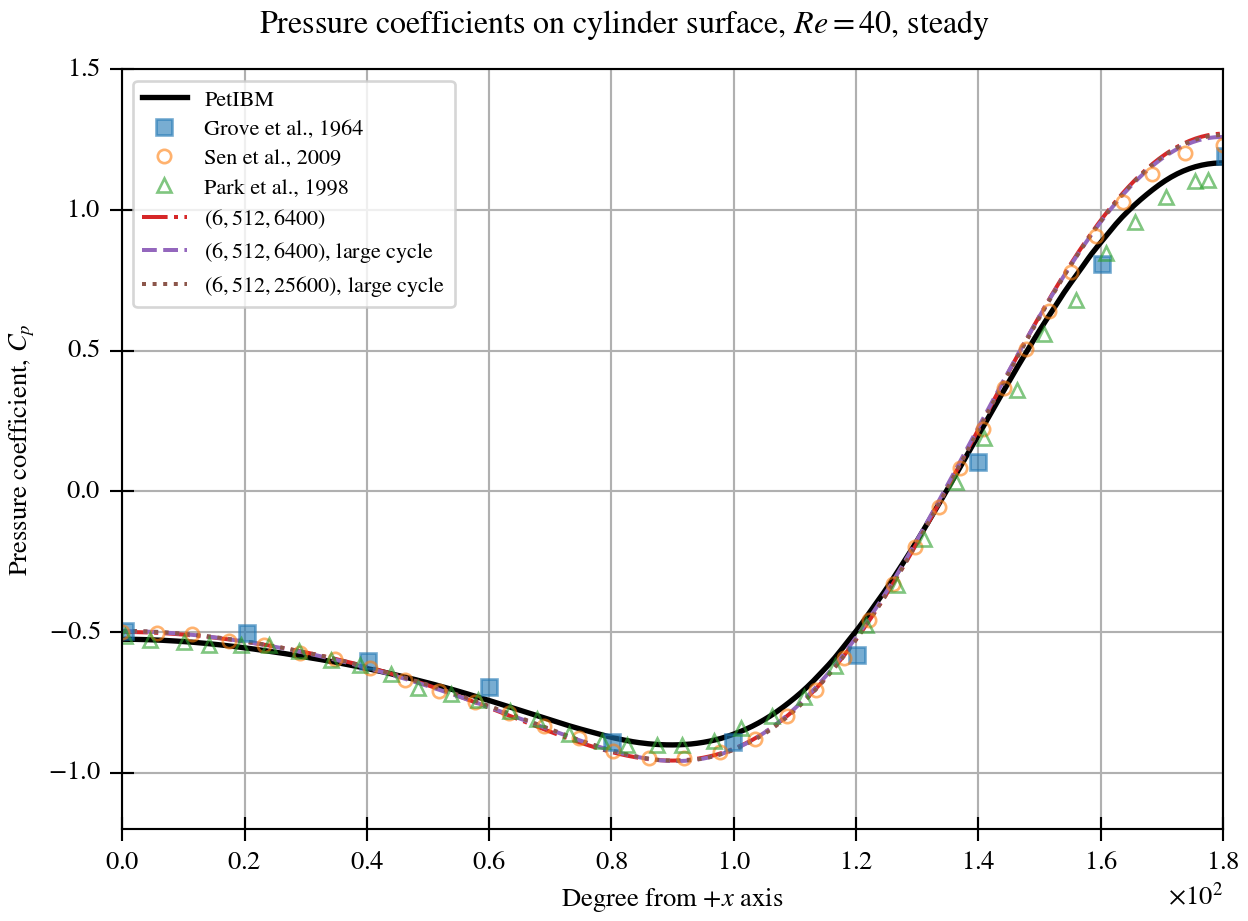
\includegraphics[width=0.9\linewidth]{cylinder-2d-re40/surface-pressure-steady}
    \caption[%
        PINNs, 2D Cylinder, $Re=40$: pressure coefficients on cylinder surface for steady solvers%
    ]{
        PINNs, 2D Cylinder, $Re=40$: pressure coefficients on cylinder surface for steady solvers. %
        The data from Grove et al., 1964 are experimental, while others are computational.%
    }%
    \label{fig:cylinder-2d-re40-surface-cp-steady}
\end{figure}
\begin{figure}[hbt!]
    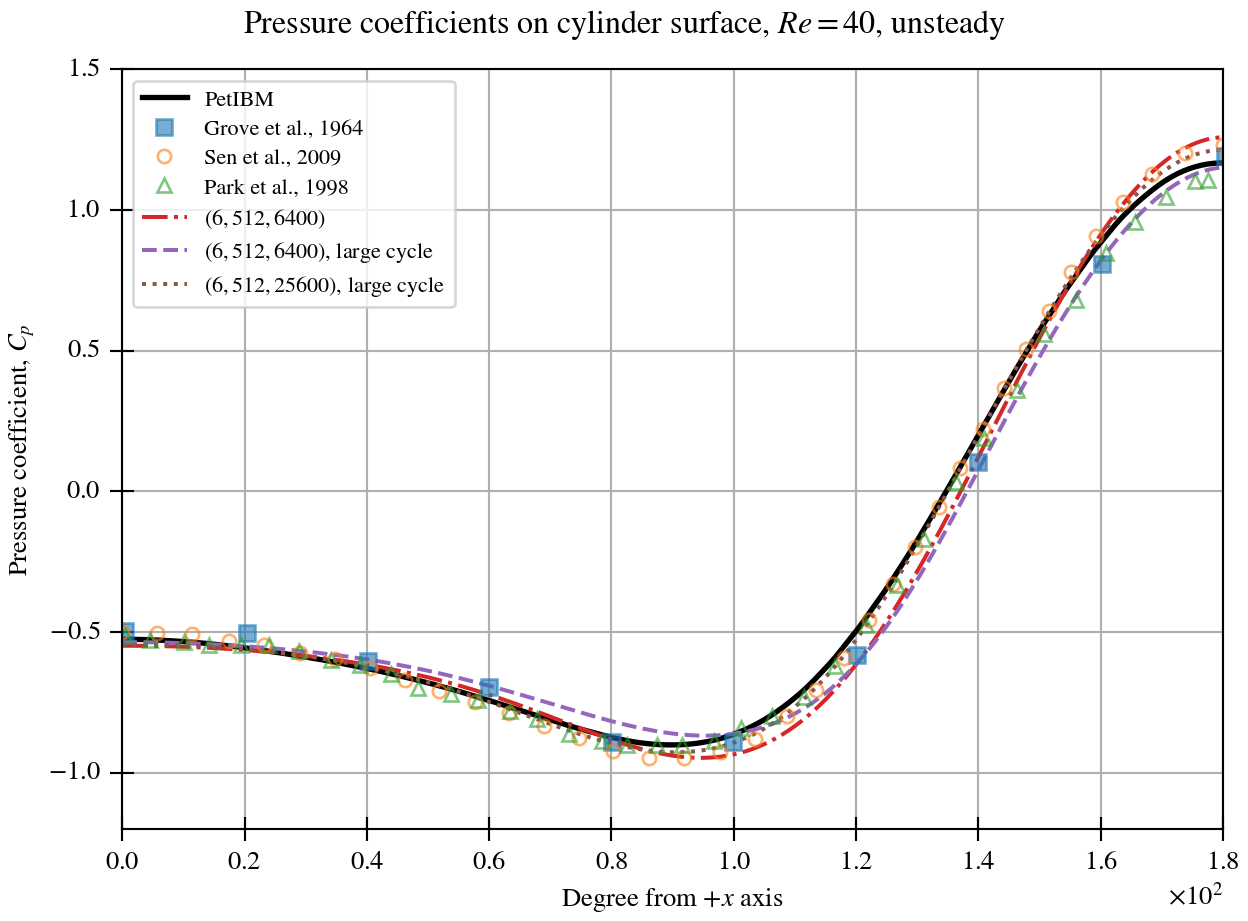
\includegraphics[width=0.9\linewidth]{cylinder-2d-re40/surface-pressure-unsteady}
    \caption[%
        PINNs, 2D Cylinder, $Re=40$: pressure coefficients on cylinder surface for unsteady solvers%
    ]{
        PINNs, 2D Cylinder, $Re=40$: pressure coefficients on cylinder surface for unsteady solvers. %
        The data from Grove et al., 1964 are experimental, while others are computational.
    }%
    \label{fig:cylinder-2d-re40-surface-cp-unsteady}
\end{figure}
As there is no correct answer, we consider the results of the surface $C_p$ validated.
All results from PINNs are visually within the range made up by the reference data.
% vim:ft=tex
